%\documentclass[]{bio}
\documentclass[oupdraft]{bio}
%\usepackage[colorlinks=true, urlcolor=citecolor, linkcolor=citecolor, citecolor=citecolor]{hyperref}

% Add history information for the article if required
\history{xxx}

\usepackage[utf8]{inputenc}
\usepackage{amsmath}
\usepackage{amsfonts}
\usepackage{amssymb}
\usepackage{amsthm}
\usepackage{graphicx}
\usepackage{todonotes}
\usepackage{natbib}
\usepackage{url}
\usepackage[boxruled,vlined,linesnumbered]{algorithm2e}
\usepackage{caption}
\usepackage{subcaption}
\usepackage{lineno}
\usepackage{tcolorbox}
\usepackage{hyperref}
\AtBeginDocument{\let\textlabel\label}
\hypersetup{colorlinks=true,linkcolor=black,citecolor=black,filecolor=black,urlcolor=black}


\captionsetup[figure]{labelfont=it,textfont={it},textfont=footnotesize}
\captionsetup[subfigure]{width=0.8\hsize,labelfont=bf,textfont=footnotesize,singlelinecheck=off,justification=raggedright,format=hang}

\theoremstyle{definition}
\newtheorem{definition}{Definition}



\author{Jonathan Rosenblatt \\ 
	Department of IE\&M and \\
	Zlotowsky Center for Neuroscience, \\
	Ben Gurion University of the Negev, Israel. 
	\and Jelle Goeman \\ 
	Department of Medical Statistics and Bioinformatics, \\
	Leiden University Medical Center, The Netherlands.
	\and Roee Gilron \\ Tel Aviv University,
	\and Roy Mukamel \\ Tel Aviv University.}


%% OPTIONAL MACRO DEFINITIONS
%\def\s{\sigma}
\newcommand{\set}[1]{\{ #1 \}} % A set
\newcommand{\indicator}[1]{\mathcal{I}{\set{#1}}} % The indicator function.
\newcommand{\reals}{\mathbb{R}} % the set of real numbers
\newcommand{\xS}{\mathcal{X}} % The feature space
\newcommand{\yS}{\mathcal{Y}} % The feature space
\newcommand{\expect}[1]{\mathbf{E}\left[ #1 \right]} % The expectation operator
\newcommand{\acc}{\mathcal{E}} 
\newcommand{\accEstim}{\hat{\mathcal{E}}} 
\newcommand{\accZ}{\hat{\mathcal{Z}}} 
\newcommand{\hyp}{\algo_{\data}} % A hypothesis
\newcommand{\hypFun}[2]{\algo_{#1}(#2)} % A hypothesis
\newcommand{\hypEstim}{\algo(\data)} %{\hat{\hyp}} % A hypothesis
\newcommand{\hypclass}{\mathcal{F}}
\newcommand{\prob}[1]{Prob( #1 )} % the probability of an event
\newcommand{\rv}[1]{\mathbf{#1}} % A random variable
\newcommand{\x}{\rv x} % The random variable x 
\newcommand{\y}{\rv y} % The random variable x 
\newcommand{\X}{\rv X} % The random variable x 
\newcommand{\Y}{\rv Y} % The random variable y
\newcommand{\gauss}[1]{\mathcal{N}\left(#1\right)} % The Gaussian distribution
\newcommand{\gaussp}[2]{\mathcal{N}_{#1}\left(#2\right)} % The Gaussian distribution
\newcommand{\mycaption}{Simulation details in Section\ref{sec:simulation_details}, except the changes in the sub-captions.}
\newcommand{\argmin}[2]{\mathop{argmin} _{#1}\set{#2}} % The argmin operator
\newcommand{\argmax}[2]{\mathop{argmax} _{#1}\set{#2}} % The argmin operator
\newcommand{\R}{\textsf{R }}
\newcommand{\algo}{\mathcal{A}}
\newcommand{\data}{\mathcal{S}}
\newcommand{\measure}{\mathcal{P}}
\newcommand{\measuren}{\measure_\data}
\newcommand{\union}{\cup}
\newcommand{\intersect}{\cap}
\newcommand{\majority}{\accEstim_{Maj}}
\newcommand{\statistic}{\mathcal{T}}


%\usepackage[nomarkers,nolists]{endfloat}


\begin{document}

% Title of paper
\title{Better-Than-Chance Classification for Signal Detection-- Supplementary Material}

\author{Jonathan D. Rosenblatt$^\ast$ \\ 
	\textit{Department of IE\&M and Zlotowsky Center for Neuroscience, 
		Ben Gurion University of the Negev, Israel.} 
	\\ Yuval Benjamini \\
	\textit{Department of Statistics, Hebrew University, Israel}	
	\\ Roee Gilron \\ 
	\textit{Movement Disorders and Neuromodulation Center, University of California, San Francisco.}
	\\ Roy Mukamel \\ 
	\textit{School of Psychological Science Tel Aviv University, Israel.}
	\\ Jelle Goeman \\ 
	\textit{Department of Medical Statistics and Bioinformatics, Leiden University Medical Center, The Netherlands.}
}


% Running headers of paper:
\markboth%
% First field is the short list of authors
{J.D.Rosenblatt and others}
% Second field is the short title of the paper
{Classification for detection}

\maketitle

% Add a footnote for the corresponding author if one has been
% identified in the author list
\footnotetext{johnros@bgu.ac.il}


\section{Large Sample}

We have focused on the him-dim--small-sample setup because it is appropriate for many problems in neuroimaging and genetics. 
To show that our conclusions are not due to the \emph{small-sample}, but rather, to the \emph{high-dim}, we scale our basic setup ten-fold. 
Fixing $p/n$, we simulate with $p=230$ and $n=400$. 
The results, reported in Figure~\ref{fig:large-sample}, are qualitatively similar to the high-dim--small-sample in the main text.
In particular with respect to the dominance of two-group tests. 
\begin{figure}[h]
	\centering
	\includegraphics[width=0.45\columnwidth]{"file1"}
	\caption{\textbf{Large sample}: The basic simulation setup scaled ten-fold: $n=400; p=230$.
	$\SNR$ was set to $0$ (red circle), $100$ (green triangle), $400$ (blue square) for comparable power to other simulations.}
	\label{fig:large-sample}
\end{figure}





%%%% Sphericity
\section{Departure From Sphericity}
In the main text we have departed from the sphericity assumption by allowing $\Sigma$ to be an $AR(1)$ covariance. 
We now try other covariance structures: a long-memory Brownian motion correlation, and an arbitrary (random) covariance structure. 
As seen in Figures \ref{fig:dependence_2} and \ref{fig:dependence_3}, the findings in the main test hold also for the ``long-memory'', and ``arbitrary'' correlation structures.
In particular: two-group tests dominate accuracy tests, and signal in the low PCs of the noise is masked. 



\begin{figure}[h]
	\centering
	\begin{subfigure}[t]{.45\columnwidth}
		\centering
		\includegraphics[width=1\columnwidth]{"file22"}
		\caption{Signal in direction of highest variance PC of $\Sigma$.} 
		\label{fig:dependence_21}
	\end{subfigure}
	\begin{subfigure}[t]{.45\columnwidth}
		\centering
		\includegraphics[width=1\columnwidth]{"file23"}
		\caption{Signal in direction of lowest lowest variance PC of $\Sigma$.} 
		\label{fig:dependence_22}
	\end{subfigure}
	\caption{Long-memory Brownian motion correlation: $\Sigma=D^{-1} R D^{-1}$ where $D$ is diagonal with $D_{jj}=\sqrt{R_{jj}}$, and $R_{k,l}=\min\{k,l\}$.}	
	\label{fig:dependence_2}
\end{figure}



\begin{figure}[h]
	\centering
	\begin{subfigure}[t]{.45\columnwidth}
		\centering
		\includegraphics[width=1\columnwidth]{"file18"}
		\caption{Signal in direction of highest variance PC of $\Sigma$.} 
		\label{fig:dependence_31}
	\end{subfigure}
	\begin{subfigure}[t]{.45\columnwidth}
		\centering
		\includegraphics[width=1\columnwidth]{"file17"}
		\caption{Signal in direction of lowest variance PC of $\Sigma$.} 
		\label{fig:dependence_32}
	\end{subfigure}
	%	\begin{subfigure}[t]{.3\columnwidth}
	%		\centering
	%		\includegraphics[width=1\columnwidth]{"file19"}
	%		\caption{Signal in direction of identity vector.} 
	%		\label{fig:dependence_33}
	%	\end{subfigure}
	\caption{Arbitrary Correlation. 
		$\Sigma=D^{-1} R D^{-1}$ where $D$ is diagonal with $D_{jj}=\sqrt{R_{jj}}$, and $R=A'A$ where $A$ is a Gaussian $p\times p$ random matrix with independent $\mathcal{N}(0,1)$ entries.
	}
	\label{fig:dependence_3}
\end{figure}






\section{Departure From Shift Alternatives}

Shift alternatives are the most common signal model in the univariate statistical literature. 
They are also very common in the multivariate literature, as they are implied by Fisher's LDA problem setup, known as \emph{Gaussian Bayes} in the machine learning literature.
On the other hand, effects may manifest themselves in many ways, not necessarily in location. 
We now verify our claims in models which are not ``pure shifts''. 
These include logistic regression, and a mixture class. 


\subsection{Logistic Regression}

In Figure~\ref{fig:logistic-main-and-interactions} we report the usual power simulation, when generating from a logistic regression setup with both main effects, and second order interactions.
This setup is also reported in the main text.

Formally, the logistic assumption implies that 
$P(y=1|x)=\exp(\eta)/[1+\exp(\eta)]$.
Main-effects and second order interactions imply that 
$\eta=\beta_0+x'\beta +x'Bx$, for some $p$-vector $\beta$, and symmetric $p \times p$ matrix $B$.
We also assume $x \sim \mathcal{N}(0,I_{p\times p})$.
We perform the various tests in the original space, $x$, but also in the $276$~dimensional space of main effects and second order interactions: 
$$\tilde{x}:=\Phi(x)=(x_1,\dots,x_j,\dots,x_p,\dots,x_1x_1,\dots x_jx_{j'},\dots,x_p x_p).$$

From Figure~\ref{fig:logistic-main-and-interactions} we learn that two-group tests dominate accuracy tests also in the logistic setup.
Was this to be expected, given our conclusions on multivariate shifts?
In the logistic setup $x_1$ cannot be a shifted version of $x_0$, but their means certainly differ. 
The larger the main effects, the larger the difference in means.
This suggests that a main-effect-only model ($B=0$) will be roughly similar to a shift class, and a second-order-interactions-only model may be very different than a shift class.
To isolate these two cases, we simulate a main-effects-only setup (Fig.\ref{fig:logistic-main-only}), and an interaction-only setup (Fig.\ref{fig:logistic-interactions-only}).


The main-effect-only case in Figure~\ref{fig:logistic-main-only} is not very surprising: 
the groups differ in their first moment, so that our conclusions are almost identical to the ``pure shift'' examples in the main text.
Analyzing the data in the augmented $276$ dimensional space decreases power, since the problem increases in dimension, and many more parameters need to be estimated. 

It may also be surprising that in the original space, $x$, signal detection is easier in the absence of second order interactions. 
Put differently, all tests have more power when $B=0$ than when $B \neq 0$ (Fig.\ref{fig:interactions-in-original-space} vs. Fig.\ref{fig:main-only-original-space}). 
Why does more signal/effects reduce power? 
The signal added is not in the span of the $x$ space, so for detection algorithms operating in $x$ (not $\tilde{x}$), this is actually part of the noise. 
This intuition is confirmed when analyzing in $\tilde x$: it is indeed easier to detect signal with interactions, than main effects only (Fig.\ref{fig:interactions-in-augmented-space} vs. Fig.\ref{fig:main-only-augmented-space}).

The second-order-interactions-only case in Figure~\ref{fig:logistic-interactions-only} is of particular interest. 
From Figure~\ref{fig:quadratic-form} we see that in this setup $x_1$ is roughly a scaled version of $x_0$.
In the context of machine-learning, and in particular learning in kernel spaces, this is sometimes known as a \emph{ring problem}.
When all signal is in the scatter of the distribution, we expect that tests for shifts would have poor performance. 
This intuition is confirmed: in the original space $x_0$ and $x_1$ have the same location and shift detectors have no power at all (Fig.\ref{fig:logistic-interactions-only-original}). 
In the augmented space, $x_0$ and $x_1$ differ in location so that shift detectors are re-powered (Fig.\ref{fig:logistic-interactions-only-augmented}). 
Most importantly for practitioners, the high-dim GOF tests detect the change in scatter in all these cases. 
Why the GOF tests perform so much better in the augmented space may be the topic of future research.


\begin{figure}[th]
	\centering
	\begin{subfigure}[t]{.45\columnwidth}
		\centering
		\includegraphics[width=1\columnwidth]{"file41"}
		\caption{Data analyzed in the original space ($x$).}
		\label{fig:interactions-in-original-space}
	\end{subfigure}
	\begin{subfigure}[t]{.45\columnwidth}
		\centering
		\includegraphics[width=1\columnwidth]{"file45"}
		\caption{Data analyzed in augmented interactions space ($\tilde x$).}
		\label{fig:interactions-in-augmented-space}
	\end{subfigure}
	\caption{\textbf{Logistic regression. Main effects and interactions.} 
		Data generated via $y|x \sim Binom(1,p(x));
		p(x)=\exp(\eta)/[1+\exp(\eta)];
		\eta=\beta_0 + x'\beta + x'Bx$ where 
		$\beta$ is a scaled vector of ones, 
		$B$ a scaled identity matrix, and $\beta_0$ set so that the median $\eta \approx0$.
		Finally, $x\sim \mathcal{N}(0,I_{p\times p})$. } 
	\label{fig:logistic-main-and-interactions}
\end{figure}





\begin{figure}[th]
	\centering
	\begin{subfigure}[t]{.45\columnwidth}
		\centering
		\includegraphics[width=1\columnwidth]{"file40"}
		\caption{Data analyzed in the original space ($x$).}
		\label{fig:main-only-original-space}
	\end{subfigure}
	\begin{subfigure}[t]{.45\columnwidth}
		\centering
		\includegraphics[width=1\columnwidth]{"file44"}
		\caption{Data analyzed in augmented interactions space ($\tilde x$).}
		\label{fig:main-only-augmented-space}
	\end{subfigure}
	\caption{\textbf{Logistic Regression. Main effects only.} 
	Data generated via $y|x \sim Binom(1,p(x));
	p(x)=\exp(\eta)/[1+\exp(\eta)];
	\eta=\beta_0+x'\beta$ where 
	$\beta$ is a scaled vector of ones, and $\beta_0$ set so that the median $\eta \approx0$.
	Finally, $x\sim \mathcal{N}(0,I_{p\times p})$. } 
	\label{fig:logistic-main-only}
\end{figure}



\begin{figure}[th]
	\centering
	\begin{subfigure}[t]{.3\columnwidth}
		\centering
		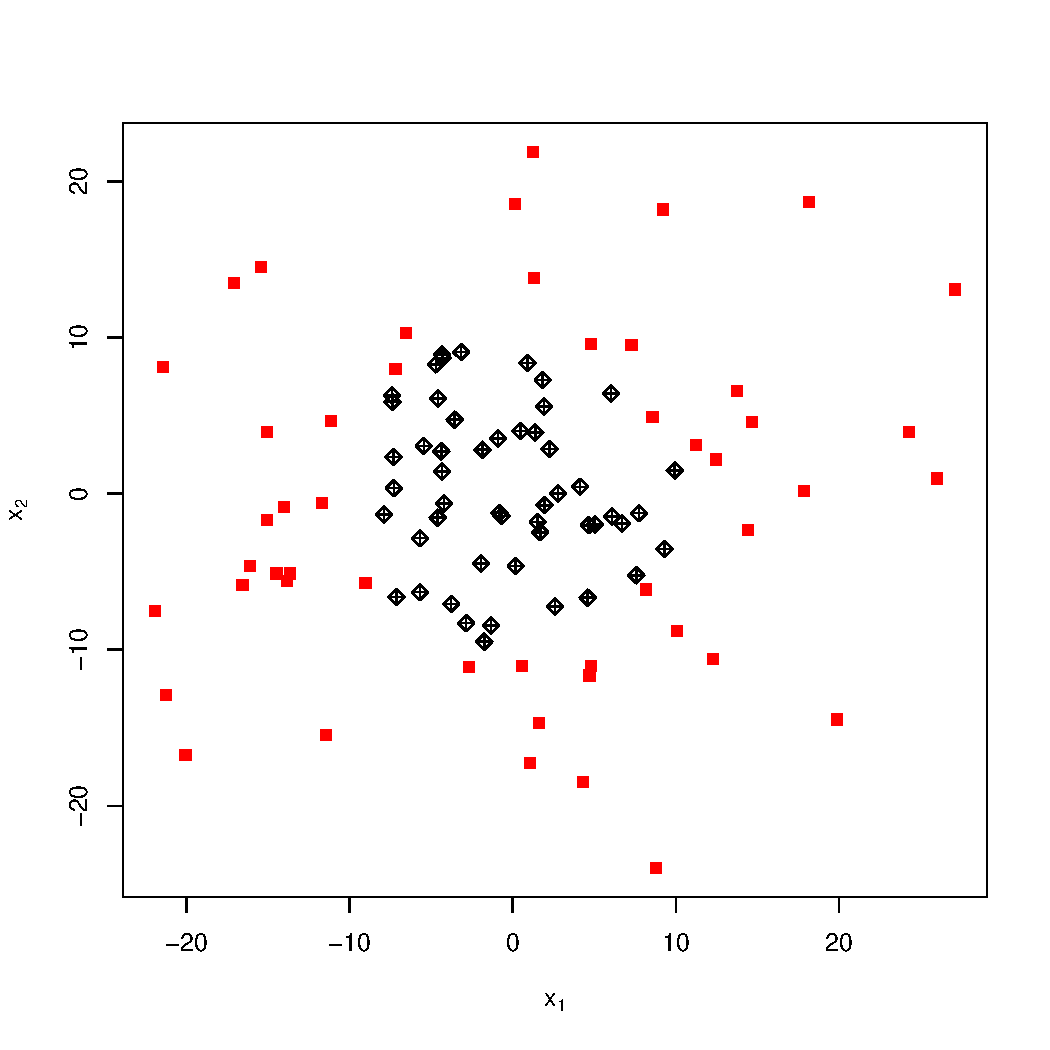
\includegraphics[width=1\linewidth]{quadratic-form}
		\caption{
			Illustration with $p=2$. 
			$y=1$ in red squares. 
			$y=0$ in black diamonds.}
		\label{fig:quadratic-form}
	\end{subfigure}
	\begin{subfigure}[t]{.3\columnwidth}
		\centering
	\includegraphics[width=1\columnwidth]{"file42"}
	\caption{Detection power in \textbf{original} space.} 
	\label{fig:logistic-interactions-only-original}
	\end{subfigure}
	\begin{subfigure}[t]{.3\columnwidth}
	\centering
	\includegraphics[width=1\columnwidth]{"file43"}
	\caption{Detection power in \textbf{augmented} space.} 
	\label{fig:logistic-interactions-only-augmented}
	\end{subfigure}
	\caption{\textbf{Logistic regression. Second order interactions only.}
		Data generated via $y|x \sim Binom(1,p(x));
		p(x)=\exp(\eta)/[1+\exp(\eta)];
		\eta=\beta_0+x'Bx$ 
		where $B$ is a scaled identity matrix.
		Finally, $x\sim \mathcal{N}(0,I_{p\times p})$.	
	}
	\label{fig:logistic-interactions-only}
\end{figure}







\subsection{Mixture Class}

Another example where $x_1$ is not a shifted version of $x_0$ is a mixture class. 
\cite{golland_permutation_2003} and \cite{golland_permutation_2005} study accuracy-tests using simulation, neuroimaging data, genetic data, and analytically.
The finite Vapnik–Chervonenkis dimension requirement \cite[Sec 4.3]{golland_permutation_2005} implies a the problem is low dimensional and prevents the permutation p-value from (asymptotically) concentrating near $1$. 
They find that the power increases with the size of the test set.
This is seen in Fig.4 of \cite{golland_permutation_2005}, where the size of the test-set, $K$, governs the discretization. 
We attribute this to the reduced discretization of the accuracy statistic.

When discussing the power of the resubstitution accuracy, \cite{golland_permutation_2005} simulate power by sampling from a Gaussian mixture family of models. 
Under their model (with some abuse of notation)
\begin{align*}
\begin{split}
x_1 & \sim \pi \gauss{\mu_1,I}+ (1-\pi) \gauss{\mu_2,I}, \\
x_0 & \sim (1-\pi) \gauss{\mu_1,I}+ \pi \gauss{\mu_2,I}.
\end{split}
\end{align*}
Varying $\pi$ interpolates between the null distribution $(\pi=0.5)$ and a shift model $(\pi=0)$. 
We now perform the same simulation as \cite{golland_permutation_2005}, but in the same dimensionality of our previous simulations.
We re-parameterize so that $\pi=0$ corresponds to the null model:
\begin{align}
\begin{split}
\label{eq:mixture_alternative}
x_1 & \sim (1/2-\pi) \gauss{\mu_1,I}+ (1/2+\pi) \gauss{\mu_2,I}, \\
x_0 & \sim (1/2+\pi) \gauss{\mu_1,I}+ (1/2-\pi) \gauss{\mu_2,I}.	
\end{split}
\end{align}
From Figure~\ref{fig:file12}, we see that for the mixture class of \cite{golland_permutation_2005} location tests are still preferred over accuracy-tests. 


\begin{figure}[h]
	\centering
	\includegraphics[width=0.5\columnwidth]{"file12"}
	\caption{\textbf{Mixture Alternatives.} $\x_i$ is distributed as in Eq.(\ref{eq:mixture_alternative}). 
		$\mu$ is a $p$-vector with $3/\sqrt{p}$ in all coordinates.
		The effect, $\pi$, is color and shape coded and varies over $0$ (red circle), $1/4$ (green triangle) and $1/2$ (blue square). }
	\label{fig:file12}
\end{figure}






\section{Sparse Alternatives}
\label{sec:sparse}

In our set of simulations we discussed ``dense'' alternatives.
Dense alternatives are motivated by neuroimaging where most brain locations in a region carry signal.
In a genetic application, a sparse alternative may be more plausible. 
Figure~\ref{fig:sparse} reports power when $\mu$ is sparse. 
As usual, two-group tests dominate accuracy-tests, only this time, the winners are not the $T^2$ type statistics, but rather, the tests for sparse shifts (\emph{Cai}, \emph{Simes}).

\begin{figure}[h]
	\centering
	\centering
	\includegraphics[width=0.5\columnwidth]{"file34"}
	\caption{Sparse $\mu$.}  
	\label{fig:sparse}	
\end{figure}





\section{Departure from Homoskedasticity and Scalar Invariance}

In our simulations variables have unit variance. 
Practitioners are already accustomed to z-score features before learning a regularized predictor (e.g. ridge regression) so this is not an unrealistic setup.
Implicit z-scoring is sometime an integral part of a test statistic. 
This is known as \emph{scalar invariance}.
The \emph{Srivastava} statistic, for instance, is scalar invariant. 
It can be (roughly) thought of as the $l_2$ norm of the $p$-vector of coordinate-wise t-statistics.
The \emph{Goeman} statistic, for instance, is not scalar invariant. 
It can be (roughly) thought of as the $l_2$ norm of the $p$-vector of variable-wise mean differences.
Under heteroskedasticity, the \emph{Goeman} statistic will give less importance to signal in the high-variance directions than signal in the low-variance directions. 
\emph{Srivastava} will give all coordinates the same importance.

In Figure~\ref{fig:heteroskedastic_11} we can see the difference between the \emph{Goeman} statistic, and the scalar-invariant \emph{Srivastava} statistic. 
We also see that two-group tests dominate accuracy-tests also in the heteroskedastic case. 

\begin{figure}[h]
	\centering
	\begin{subfigure}[t]{.45\columnwidth}
		\centering
		\includegraphics[width=1\columnwidth]{"file26"}
		\caption{$\mu$ in the high variance PC of $\Sigma$.}  
		\label{fig:heteroskedastic_11}	
	\end{subfigure}
	\begin{subfigure}[t]{0.45\columnwidth}
		\centering
		\includegraphics[width=1\columnwidth]{"file24"}
		\caption{$\mu$ in the low variance PC of $\Sigma$.}  
		\label{fig:heteroskedastic_12}	
	\end{subfigure}
	\caption{Heteroskedasticity: $\Sigma$ is diagonal with $\Sigma_{jj}=j$.}	
	\label{fig:heteroskedastic}	
\end{figure}




\section{Tie Breaking}
\label{sec:ties}

Discrete test statistics lose power by not exhausting the permissible false positive rate. 
A common remedy is a \emph{randomized test} with tie-breaking, in which the rejection of the null is decided at random in a manner that exhausts the false positive rate. 
Formally, denoting by $\mathcal{T}$ the observed test statistic, by $\mathcal{T}_\pi$, its value after under permutation $\pi$, and by $\mathbb{P}\{A\}$ the proportion of permutations satisfying $A$ then the randomized version of our tests imply that if the permutation p-value, 
$\mathbb{P}\{\mathcal{T}_\pi \geq \mathcal{T}\}$, 
is greater than  $\alpha$ then we reject the null with probability 
$$ max\left\{\frac{\alpha - \mathbb{P}\{\mathcal{T}_\pi > \mathcal{T}\}}{\mathbb{P}\{\mathcal{T}_\pi = \mathcal{T}\}},0 \right\}.$$

Figure~\ref{fig:file33} reports the basic simulation setup while allowing for random tie breaking. 
It demonstrates that the power disadvantage of accuracy-tests cannot be remedied by random tie breaking.

\begin{figure}[ht]
	\centering
	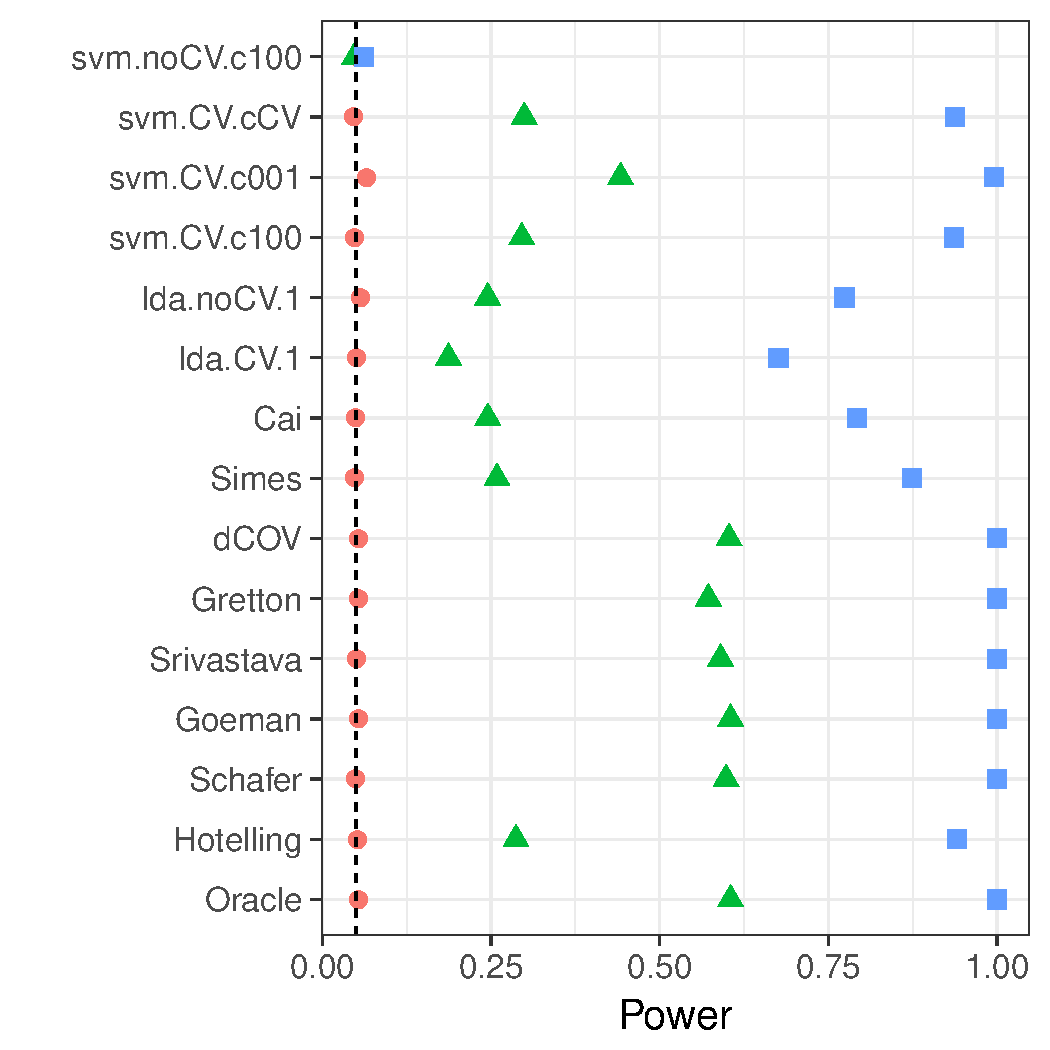
\includegraphics[width=0.5\columnwidth]{file33}
	\caption{\textbf{Tie breaking}: The basic simulation setup with random tie breaking.}
	\label{fig:file33}
\end{figure}




\section{Fixed SNR}
\label{sec:fix_snr}

For a fair comparison between simulations, in particular between those with different $\Sigma$, we needed to fix the difficulty of the problem.
We fix the Kullback–Leibler Divergence between distributions of sample means. 
Formally, the Kullback–Leibler Divergence between two Gaussian populations is given by 
\begin{align}
\label{eq:KLD}
KL[x_1,x_0]=\frac{1}{2}\left(
\log \frac{\det \Sigma_0}{\det \Sigma_1}-p+Tr(\Sigma_0^{-1}\Sigma_1)+(\mu_0-\mu_1)'\Sigma^{-1}_0(\mu_0-\mu_1)
\right),
\end{align}
where $x_y\sim\mathcal{N}(\mu_y,\Sigma_y)$.
In the case of the sample means of two shifted groups of size $n$, then 
\begin{align}
\label{eq:mahalanobis}
KL[\bar x_1,\bar x_0]=
\frac{n}{2}\mu'\Sigma^{-1}\mu=
\frac{n}{2}\Vert \mu \Vert_\Sigma^2,
\end{align}
where $\mu:=\mu_1-\mu_0$. 

In most of our simulations we fixed $n \Vert \mu \Vert_\Sigma^2$. 
The logistic regression setup is an exception because the signal is not a shift. 
We did set effect sizes so that power in the logistic regression is comparable to power in the other examples.

Fixing $n \Vert \mu \Vert_\Sigma^2$ implies that the Euclidean norm of $\mu$ varies with $\Sigma$, with the sample size, and with the direction of the signal.
An initial intuition may suggest that detecting signal in the low variance PCs is easier than in the high variance PCs. 
This is true when fixing $\Vert \mu \Vert_2$, but not when fixing $\Vert \mu \Vert_{\Sigma}$.

For completeness, Figure~\ref{fig:dependence_4} reports the power analysis under $AR(1)$ correlations, but with $\Vert \mu \Vert_2$ fixed.
We compare the power of a shift in the direction of some high variance PC (Figure~\ref{fig:dependence_41}), versus a shift in the direction of a low variance PC (Figure~\ref{fig:dependence_42}).
The intuition that it is easier to detect signal in the low variance directions is confirmed. 

\begin{figure}[h]
	\centering
	\begin{subfigure}[t]{.45\columnwidth}
		\centering
		\includegraphics[width=1\columnwidth]{"file32"}
		\caption{$\mu$ in PC7 of $\Sigma$.}  
		\label{fig:dependence_41}	
	\end{subfigure}
	\begin{subfigure}[t]{0.45\columnwidth}
		\centering
		\includegraphics[width=1\columnwidth]{"file31"}
		\caption{$\mu$ in PC15 of $\Sigma$.}  
		\label{fig:dependence_42}	
	\end{subfigure}
	\caption{Short memory, AR(1) correlation. $\Vert \mu \Vert_2$ fixed. }	
	\label{fig:dependence_4}		
\end{figure}

Other authors have also observed the need for fixing the SNR for a fair comparison between tests.
In \cite{ramdas2015decreasing}, authors prefer to use sparse alternatives.
With sparse alternatives, the difficulty of the problem is governed by the sparsity of the signal and not only the dimension of the data. 
In \cite{chen2010two}, authors fix $\Vert \mu \Vert_2^2/\Vert \Sigma \Vert^2_{Frob}$ where $\Vert \Sigma \Vert^2_{Frob}=\Tr(\Sigma'\Sigma)$ is the Frobenius matrix norm. 
Clearly, $\Vert \mu \Vert_2^2/\Vert \Sigma \Vert^2_{Frob}$ is invariant to the direction of the signal with respect to the noise. 
For this reason, we prefer fixing $\Vert \mu \Vert_\Sigma$.












\newpage
\bibliographystyle{abbrvnat}
\bibliography{Permuting_Accuracy.bib}

\end{document}

